\documentclass[a4paper]{cernatsnote}
\usepackage{graphicx}
\usepackage{listings}
\usepackage{caption}
\usepackage{listings}
\usepackage{parskip}
\usepackage{hyperref}

\usepackage[usenames,dvipsnames]{xcolor}

\definecolor{dkgreen}{rgb}{0,0.6,0}
\definecolor{gray}{rgb}{0.5,0.5,0.5}
\definecolor{mauve}{rgb}{0.58,0,0.82}
\definecolor{Brown}{cmyk}{0,0.81,1,0.60}
\definecolor{OliveGreen}{cmyk}{0.64,0,0.95,0.40}
\definecolor{CadetBlue}{cmyk}{0.62,0.57,0.23,0}

\definecolor{amber}{rgb}{1.0, 0.49, 0.0}
\definecolor{azure}{rgb}{0.0, 0.5, 1.0}
\definecolor{brandeisblue}{rgb}{0.0, 0.44, 1.0}
\definecolor{fluorescentpink}{rgb}{1.0, 0.08, 0.58}
\definecolor{lime}{rgb}{0.0, 1.0, 0.0}

\lstset{ 
	backgroundcolor	=	\color{white},  				% choose the background color; you must add \usepackage{color} or \usepackage{xcolor}
	basicstyle		=	\footnotesize,       				% the size of the fonts that are used for the code
	%basicstyle	=	\normalsize,
	breakatwhitespace=	false,       					% sets if automatic breaks should only happen at whitespace
	breaklines		=	true,               				% sets automatic line breaking
	captionpos		=        b,                   				% sets the caption-position to bottom
	commentstyle	=	\color{dkgreen},  				% comment style
	% deletekeywords	=	{...},        					% if you want to delete keywords from the given language
	escapeinside	=	{\%*}{*)},         				% if you want to add LaTeX within your code
	%extendedchar	=	true,              				% lets you use non-ASCII characters; for 8-bits encodings only, does not work with UTF-8
	frame			=	ltrb,                  				% adds a frame around the code
	framesep		=	5pt,
	identifierstyle	=	\ttfamily \color{black}\bfseries,
	keywordstyle	=	\ttfamily \color{blue},      		% keyword style
	language		=	Bash,                				% the language of the code
	morekeywords	=	{*,...},           				% if you want to add more keywords to the set
	numbers			=	left,                   				% where to put the line-numbers; possible values are (none, left, right)
	numbersep		=	5pt,                  				% how far the line-numbers are from the code
	numberstyle		=	\tiny\color{gray},  				% the style that is used for the line-numbers
	rulecolor		=	\color{black},        				% if not set, the frame-color may be changed on line-breaks within not-black text (e.g. comments (green here))
	showspaces		=	false,               				% show spaces everywhere adding particular underscores; it overrides 'showstringspaces'
	showstringspaces	=	false,         					% underline spaces within strings only
	showtabs		=	false,                 				% show tabs within strings adding particular underscores
	stepnumber		=	2,                  				% the step between two line-numbers. If it's 1, each line will be numbered
	stringstyle		=	\ttfamily\color{gray},      		% string literal style
	tabsize			=	2,                      				% sets default tabsize to 2 spaces
	title			=	\lstname                  				% show the filename of files included with \lstinputlisting; also try caption instead of title
}

% Base classes
\lstset{
	emph		=	{mkdir, cp, ln, ssh, module, git, curl, make},
	emphstyle		= 	\ttfamily \color{blue}
}

% User classes
\lstset{
	emph		=	{[2]User_Class, myMADInterface},
	emphstyle		= 	{[2]\ttfamily \color{amber}}
}

% Functions
\lstset{
	emph		=	{[3]Function, TreatTypeAsDrift},
	emphstyle		= 	{[3]\ttfamily \color{fluorescentpink}}
}

% Units
\lstset{
	emph		={[4]Unit, km, TeV, eV, meter}, emphstyle	=	{[4]\ttfamily \color{lime}}
}



\email{haroon.rafique@cern.ch}

\title{PyORBIT on HPC-Batch}
\documentlabel{CERN-ATS-Note-2018-??? TECH}

\author{Haroon Rafique / BE-ABP}
\keywords{PyORBIT, Space Charge, HPC, HPC-Batch, Slurm, PTC, MAD, Python}
\makeindex

\def \howtoaccess {\url{https://cern.service-now.com/service-portal/article.do?n=KB0004541}}
\def \headnode {\texttt{hpc-batch.cern.ch}}
\def \jbgithub {\href{https://github.com/jbcern/py-orbit}{https://github.com/jbcern/py-orbit.git}}
\def \hbgithub {\href{https://github.com/hannes-bartosik/py-orbit}{https://github.com/hannes-bartosik/py-orbit.git}}
\def \pyorbitgithub {\href{https://github.com/PyORBIT-Collaboration/py-orbit}{https://github.com/PyORBIT-Collaboration/py-orbit.git}}
\def \ptcgithub {\href{https://github.com/jbcern/PTC/tree/analytical-space-charge-acceleration}{https://github.com/jbcern/PTC.git}}
\def \batchroot {\texttt{\textbackslash hpcscratch\textbackslash $<$user$>$\textbackslash}}
\def \batchorbitroot {\texttt{\textbackslash hpcscratch\textbackslash $<$user$>$\textbackslash PyORBIT\textbackslash}}
\def \batchorbitptc {\texttt{\textbackslash hpcscratch\textbackslash $<$user$>$\textbackslash PyORBIT\textbackslash py-orbit\textbackslash ext\textbackslash PTC\textbackslash}}
\def \pyorbiteos {\texttt{\textbackslash eos\textbackslash project\textbackslash p\textbackslash pyorbit\textbackslash public\textbackslash HPC-Batch\textbackslash}}
\def \slurm {\href{https://slurm.schedmd.com/}{https://slurm.schedmd.com/}}
\def \slurmman {\href{https://slurm.schedmd.com/man_index.html}{https://slurm.schedmd.com/man\_index.html}}

\begin{document}
	
\maketitle % this produces the title block

\begin{abstract}
	A batch HPC cluster using the \href{https://slurm.schedmd.com/}{Slurm} (Simple Linux Utility for Resource Management) workload manager has been set up for users of \href{https://www.open-mpi.org/}{MPI} (Message Passing Interface) applications that are massively parallel and computationally intensive. Access is restricted to approved HPC (High Performance Computing) users, mainly from the Accelerator and Technology sector. 
	
	PyORBIT, a Python/C++ implementation of the ORBIT (Objective Ring Beam Injection and Tracking) code used at CERN for space charge simulations, is well suited to this system. Instructions are provided for installing and running PyORBIT on the HPC-Batch system.
\end{abstract}

%%%%%%%%%%%%%%%%%%----------------------------------------------------------------------------------------
%% INTRODUCTION %%
%%%%%%%%%%%%%%%%%%----------------------------------------------------------------------------------------	
\section{Introduction}
\label{sec:intro}
	
Official instructions for accessing the HPC-Batch system are available in the knowledge base article \href{https://cern.service-now.com/service-portal/article.do?n=KB0004541}{KB0004541}: "How to access and use the batch HPC cluster":

\texttt{\howtoaccess}

These instructions are repeated and expanded upon here. 
	
%% Hardware %%
%%%%%%%%%%%%%%------------------------------------------------------------------------------------------			
\subsection{Hardware}

\begin{table}
	\begin{center}
		\begin{tabular}[!b]{|l|c|c|}
			\hline
			\textbf{Queue} 			& \textbf{Nodes} & \textbf{Time Limit} \\
			\hline
			\textbf{batch-short}	& 10			  & 2 days (2-00:00:00) \\
			\textbf{batch-long}		& 66			  & $\infty$ \\
			\textbf{be-short}		& 69			  & 2 days (2-00:00:00) \\
			\textbf{be-long}		& 72			  & $\infty$ \\
			\hline
		\end{tabular}
		\caption{Computing resources and job time limits on HPC-Batch.}
		\label{tab:cpus}
	\end{center}
\end{table}

Table~\ref{tab:cpus} shows the available resources on HPC-Batch. There are a total of 217 nodes, each with 20 physical CPUs, and each viewed as 2 cores due to hyperthreading, totalling 8680 `cores' (or 4340 physical cores). The nodes are split into four queues, two short (2 day limit), and two long (infinite limit). The `batch' queues may be used by all, and the `be' queues are reserved for members of BE (beams department).

HPC-Batch should not replace HTCondor or standard lxplus simulations, instead it should be used for massively parallel computationally intense simulations where required.

Unfortunately it is non-trivial to call simulation input files, or in fact executables, from AFS in a reliable manner. Instead one must install PyORBIT on ones HPC-Batch scratch space \texttt{\textbackslash hpcscratch\textbackslash $<$user$>$}, and copy all simulation data to this local directory. When the simulation is complete, it is recommended that the user copies all important output back to AFS or to EOS, as the scratch space is not backed up. This cannot be done within the submission script, and must be done manually, or in a separate script called by the user (i.e. not called from within the submission script).

%% Accessing HPC-Batch %%
%%%%%%%%%%%%%%%%%%%%%%%%%---------------------------------------------------------------------------------			
\subsection{Accessing HPC-Batch}
\label{sec:access}

In order to gain access to the HPC-Batch system please request access to the e-group \href{https://e-groups.cern.ch/e-groups/Egroup.do?egroupId=10245625&AI_USERNAME=HARAFIQU&searchField=0&searchMethod=0&searchValue=service-hpc-be&pageSize=30&hideSearchFields=false&searchMemberOnly=false&searchAdminOnly=false&AI_SESSION=lKFyHz8s-iVcgi9UtzwK-aBtk4OSxot37tlEfn8KCeHPzfMElLZd!393472965!1522333073243}{service-hpc-be} via e-groups or email \texttt{abp-cwg-admin@cern.ch}.

To access HPC-Batch one must log in to the head node \headnode, replacing $<$user$>$ with ones CERN account user name:

\begin{lstlisting}[language=bash, belowskip=-3\medskipamount]
$ ssh -XY <user>@hpc-batch.cern.ch
\end{lstlisting}

To check the available modules use:
\begin{lstlisting}[language=bash, belowskip=-3\medskipamount]
$ module avail
\end{lstlisting}

The system use GCC v4 as default, this is sufficient for PyORBIT, but it can be changed to GCC v6 if required using:
\begin{lstlisting}[language=bash, belowskip=-3\medskipamount]
$ module load compiler/gcc6
\end{lstlisting}	

MPI versions may also be selected, for PyORBIT, and in general, one must initialise this using:

\begin{lstlisting}[language=bash, belowskip=-3\medskipamount]
$ module load mpi/mvapich2/2.2
\end{lstlisting}

This may be included in ones \texttt{$\sim$/.bashrc} configuration file, or ones Slurm submission script.

%%%%%%%%%%%%%%%%%%----------------------------------------------------------------------------------------
%% INSTALLATION %%
%%%%%%%%%%%%%%%%%%----------------------------------------------------------------------------------------
\section{Installing PyORBIT on HPC-Batch}
\label{sec:install}

There are currently a number of options available when installing PyORBIT. The CERN branches are made available on GitHub by Hannes Bartosik and Jean-Baptiste Lagrange. The original code (developed by SNS) is also available on GitHub. Two options are provided, the first is using Jean-Baptiste Lagrange's versions of PyORBIT and PTC, and the second is replacing the PyORBIT version with one of Hannes Bartosik's branches.

Jean-Baptiste Lagrange's code is located in the public repository:

\texttt{\jbgithub}

Hannes Bartosik's code is located in the public repository:

\texttt{\hbgithub}

please note that there are a number of branches; \href{https://github.com/hannes-bartosik/py-orbit/tree/new-features}{new-features} and \href{https://github.com/hannes-bartosik/py-orbit/tree/analytical-space-charge}{analytic-space-charge} are likely to be the most useful currently. These branches will all be merged in the near future.

The original PyORBIT code is also available from GitHub, but may not provide the required functionality for CERN users:

\texttt{\pyorbitgithub}

For tracking, PTC is also required. The latest version to be used for PyORBIT can be found on GitHub:

\texttt{\ptcgithub}

The \href{https://github.com/jbcern/PTC/tree/analytical-space-charge-acceleration}{analytical-space-charge-acceleration} branch provides the most up-to-date version.

PyORBIT runs within a virtual environment in order to utilise specific versions of libraries such as Python 2.7. As such one must take care of environment variables when running on HPC-Batch.

The user must locally install PyORBIT on HPC-Batch, for this step-by-step instructions are given (if facing difficulties please contact haroon.rafique, or py.orbit at cern.ch):
	
\begin{enumerate}
\item After being granted access, log into the HPC-Batch head node:
\begin{lstlisting}[language=bash, belowskip=-3\medskipamount]
$ ssh -XY <user>@hpc-batch.cern.ch
\end{lstlisting}
\item Make sure that your \texttt{\$PATH} and other environment variables in your \texttt{$\sim$/.bashrc} configuration file do not conflict with those required for PyORBIT, for example the \texttt{\$PYTHONPATH} should be empty.
\item Use the PyORBIT installation script `install\_PyORBIT.sh' given in subsection~\ref{sec:install_script}, making sure to adjust the variables as instructed in subsection~\ref{sec:install_script}. It can be copied from eos:
\begin{lstlisting}[language=bash, belowskip=-3\medskipamount]
$ cp eos/project/p/pyorbit/public/HPC-Batch/install_PyORBIT.sh .
\end{lstlisting}		
\item Create a directory in your home space \batchroot. It is strongly suggested to name this directory \texttt{PyORBIT} if you only intend to install a single version of PyORBIT and PTC. If you intend to use multiple versions then name the directory something else - for example \texttt{PyORBIT\_new\_features} and create a soft link using linux command \texttt{ln -s directory\_name link\_name} called PyORBIT, for example: 
\begin{lstlisting}[language=bash, belowskip=-3\medskipamount]
$ mkdir PyORBIT_new_features
$ ln -s PyORBIT_new_features PyORBIT
\end{lstlisting}
It is important that the name of this folder is not changed after installation, as certain virtual environment variables are set using the folder name at installation. Enter the PyORBIT directory, copy the install script here, and run it:
\begin{lstlisting}[language=bash, belowskip=-3\medskipamount]
$ mkdir PyORBIT
$ cd PyORBIT
$ cp /eos/project/p/pyorbit/public/HPC-Batch/install_PyORBIT.sh .
$ ./install_PyORBIT.sh > install_output.txt &
\end{lstlisting}
\item The installation script should take a few hours to run. It is difficult to know when it has finished as all output will be pipelined to the \texttt{`install\_output.txt'} file. Keep checking when this file has been updated, if it is within the last few minutes then the install script is still running.
\item After a few hours check that the install script has finished running, and check the \texttt{`install\_output.txt'} file in order to ascertain if the installation proceeded with no errors.
\item If no errors are present, it is usually necessary to install PTC manually. Though the install script should have pulled PTC from GitHub, it may not have been installed due to an environment variable conflict. Check the directory \batchorbitptc \texttt{obj\textbackslash}, if there are no \texttt{.o} files present, PTC has not been installed.

In this case run the \texttt{make} command in \batchorbitptc. It is likely that this will produce the following error:
\begin{lstlisting}[language=bash, belowskip=-3\medskipamount]
../../conf/make_root_config:5: /conf/make_common_config: No such file or directory
../../conf/make_root_config:25: /conf//make_root_config: No such file or directory
make: *** No rule to make target `/conf//make_root_config'. Stop.			
\end{lstlisting}		
In order to mitigate this, in the 

\batchorbitroot\texttt{\textbackslash py-orbit\textbackslash conf\textbackslash make\_root\_config} 

file, comment out lines 5 and 25 by placing a \texttt{\#} at the start of each line:
\begin{lstlisting}[language=bash, belowskip=-3\medskipamount]
include  ${ORBIT_ROOT}/conf/${ORBIT_ARCH}/make_root_config
...
include  ${ORBIT_ROOT}/conf/make_common_config
\end{lstlisting}
The intel fortran libraries are required to install PTC, so one must also execute the following source command:
\begin{lstlisting}[language=bash, belowskip=-3\medskipamount]
$ source /cvmfs/projects.cern.ch/intelsw/psxe/linux/all-setup.sh
\end{lstlisting}
		
The Makefile in the \texttt{PTC} directory should also be modified:
\begin{lstlisting}[language=bash, belowskip=-3\medskipamount]		
#------------------------------
# External 'include' locations
#------------------------------

INCLUDES += -I/hpcscratch/user/<user>/PyORBIT/include/python2.7
\end{lstlisting}		
		
Now executing the \texttt{make} command in 

\batchorbitptc 

should be successful. After installing PTC (check the 

\batchorbitptc \texttt{obj\textbackslash}

directory for \texttt{.o} files as before to confirm the installation), remember to uncomment out the lines in the configuration file.

\item[]{Once these steps are complete, PyORBIT has been installed.}		
	
\end{enumerate}	
	

%%%%%%%%%%%%%%%%%%----------------------------------------------------------------------------------------
%% SUBMISSION   %%
%%%%%%%%%%%%%%%%%%----------------------------------------------------------------------------------------	
\section{Job Submission}
\label{sec:jobsubmission}

\begin{enumerate}
\item Log into the HPC-Batch head node:
\begin{lstlisting}[language=bash, belowskip=-3\medskipamount]
$ ssh -XY <user>@hpc-batch.cern.ch
\end{lstlisting}

\item Using the \texttt{sinfo} command, check availability in the queues (see Fig.~\ref{fig:sinfo} for an example), and choose the appropriate queue for your submission. If your job should take less than 2 days, use one of the short queues, otherwise use a long queue. The `be' queues are reserved for members of the beams department at CERN, the `batch' queues may be used by any member of CERN.

\item Using the \texttt{\#BATCH} commands (see Section~\ref{sec:SlurmScriptCommands}), create a submission script in bash. For an example of this see Section~\ref{sec:JobSubmissionScript}.

\item You must copy all files related to the job to the local \texttt{\textbackslash hpcscratch\textbackslash $<$user$>$} directory. HPC-Batch is part of the AFS and EOS filesystems, though these may not (in general) be used in a submission script. Any file transfers to or from AFS or EOS must be done outside of the job (i.e. the submission script or executable).

\item Submit the job(s) using the \texttt{sbatch} command:
\begin{lstlisting}[language=bash, belowskip=-3\medskipamount]
$ sbatch submission_script.sh
\end{lstlisting}

\item You may use Slurm commands (shown in Section~\ref{sec:SlurmCommands}) to observe the progress of your submission.

\item When your job is complete, it is suggested that you move the output and important data to AFS or EOS. Any file transfers to or from AFS or EOS must be done outside of the job (i.e. the submission script or executable).
\end{enumerate}

%% SLURM Commands   %%
%%%%%%%%%%%%%%%%%%%%%%------------------------------------------------------------------------------------	
\subsection{Slurm Commands}
\label{sec:SlurmCommands}

The following Slurm commands may be useful when using HPC-Batch, they are described in detail on the Slurm manual pages:
\slurmman

\begin{itemize}
	\item{\textbf{squeue}} - view job and job step information, -u $<$user$>$ displays a specific users jobs.
	\item{\textbf{sacct}} - displays accounting data for all obs and job steps in the Slurm accounting log or Slurm database.
	\item{\textbf{sbatch}} - submit a batch script to Slurm.
	\item{\textbf{srun}} - run parallel jobs (used similarly to mpirun).
	\item{\textbf{scancel}} - used with a job ID to kill the specified job.
	\item{\textbf{sinfo}} - displays the status of all available nodes, an example of this command on the HPC-Batch system is given in Fig.~\ref{fig:sinfo}.
		\begin{figure}		
			\centering
			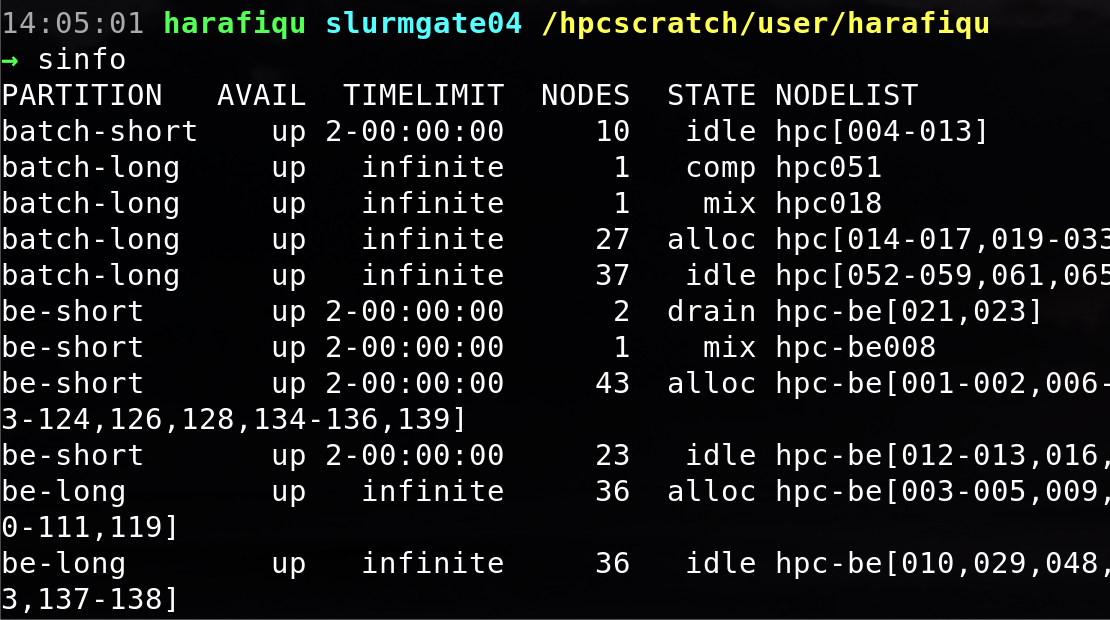
\includegraphics[width=0.8\columnwidth]{sinfo.png}
			\caption{\texttt{sinfo} command output on HPC-Batch.}
			\label{fig:sinfo}
		\end{figure}
	
\end{itemize}

%% SLURM Script Commands   %%
%%%%%%%%%%%%%%%%%%%%%%%%%%%%%------------------------------------------------------------------------------	
\subsection{Slurm Script Commands}
\label{sec:SlurmScriptCommands}

In a bash script, the following \texttt{\#SBATCH} commands may be used to specify job parameters:

\begin{itemize}
	\item{\textbf{-p}} - queue name, for HPC-Batch the options are be-short, be-long, batch-short, batch-long.
	\item{\textbf{-N}} - number of nodes, each node has threads over 20 cpus on HPC-Batch, and the number of nodes does not need to be specified, only the number of tasks.
	\item{\textbf{-n}} - number of tasks (threads).
	\item{\textbf{--job-name}} - job name.
	\item{\textbf{-t}} - wall-clock time limit for the job, in the format day-hour:minute:second, for example 1-10:00:00. This is a hard limit, if exceeded your job will be cancelled by Slurm.
	\item{\textbf{-o}} - the output file created (not from PyORBIT). This file will record what would normally be output to screen/console. A useful format is name.\%N.\%j.out, where \%N is the node number, and \%j is the Job ID.
	\item{\textbf{-e}} - the error file created (not from PyORBIT). This file will record what would normally be output to screen/console. A useful format is name.\%N.\%j.out, where \%N is the node number, and \%j is the Job ID.
	\item{\textbf{--mem}} - the RAM allocation for this job, for example 12gb.		
\end{itemize}

For the HPC-Batch system, it is necessary to specify a queue \textbf{\texttt{-p}}, the number of tasks (threads) required \textbf{\texttt{-n}}, and the time limit \textbf{\texttt{-t}}. An example use of these variables is shown below:
	
\begin{lstlisting}[language=bash, belowskip=-3\medskipamount]
#!/bin/bash
#SBATCH -p be-short
#SBATCH -n 123
#SBATCH --mem 12gb
#SBATCH --job-name TestJob
#SBATCH -t 1-23:45:01
#SBATCH -o slurm.%N.%j.out
#SBATCH -e slurm.%N.%j.err
\end{lstlisting}


%% Errors       %%
%%%%%%%%%%%%%%%%%%----------------------------------------------------------------------------------------
\subsection{Possible Job Errors}

A common cause of errors when using PyORBIT on the HPC-Batch system is the improper creation of the virtual environment on each node. 

When encountering Python errors such as \texttt{ImportError: No module named ...}, it is likely that either the node is not running the correct version of Python, or the \texttt{\$PYTHONPATH} is not correctly set. Try outputting these and making sure that they correspond to the correct directory in your PyORBIT installation. The \texttt{which python} command in a terminal will show if the system Python version is running. One must activate Python 2.7 if using PyORBIT, this is shown in Fig~\ref{fig:python}.

\begin{figure}		
	\centering
	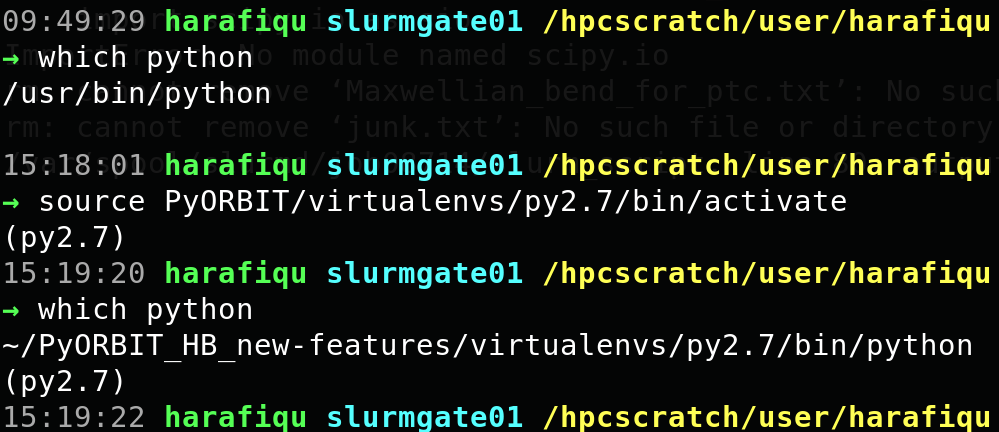
\includegraphics[width=0.8\columnwidth]{python.png}
	\caption{\texttt{which python} command output on HPC-Batch, and activation of Python 2.7, which is installed as a prerequisite for PyORBIT.}
	\label{fig:sinfo}
\end{figure}

When encountering Fortran errors, the most likely candidate is a lack of sourcing the intel Fortran libraries that are required in PTC. This should be rectified using the following command:
\begin{lstlisting}[language=bash, belowskip=-3\medskipamount]
$ source /cvmfs/projects.cern.ch/intelsw/psxe/linux/all-setup.sh
\end{lstlisting}

PyORBIT uses MPI for parallelisation, and this is done rigorously, however a user script may not properly take into account MPI concerns. For example if all threads/cores need to interact, they must all be at the same stage in the simulation. Or if one thread is creating a file that is needed by all threads, the others must wait until the file is created before reading it. When encountering MPI errors, it is suggested that these synchronisations are handled correctly.

%%%%%%%%%%%%%%%%%%----------------------------------------------------------------------------------------
%% SCRIPTS      %%
%%%%%%%%%%%%%%%%%%----------------------------------------------------------------------------------------	
\section{Scripts}
\label{sec:scripts}

A number of scripts are provided as examples or for reference.

%% HPC-Batch Custom Environment   %%
%%%%%%%%%%%%%%%%%%%%%%%%%%%%%%%%%%%%---------------------------------------------------------------------	
\subsection{HPC-Batch Custom Environment}
\label{sec:environment_script}

The following environment variables may be used independently, called from within a Slurm submission script, or incorporated into a submission script.
	
\begin{lstlisting}[language=bash, belowskip=-3\medskipamount]
#!/bin/bash
# Use the installed Python version 2.7 (required for PyORBIT)
source /hpcscratch/user/<user>/PyORBIT/virtualenvs/py2.7/bin/activate

# Set up the PyORBIT virtual environment
source /hpcscratch/user/<user>/PyORBIT/py-orbit/customEnvironment.sh

# Intel fortran libraries needed for PTC
source /cvmfs/projects.cern.ch/intelsw/psxe/linux/all-setup.sh
\end{lstlisting}

	
%% Sbatch Job Submission Script %%
%%%%%%%%%%%%%%%%%%%%%%%%%%%%%%%%%%---------------------------------------------------------------------------		
\subsection{Sbatch Job Submission Script}	
\label{sec:JobSubmissionScript}

The following bash script is an example of a Slurm batch submission script. It is run with the command:
\begin{lstlisting}[language=bash, belowskip=-3\medskipamount]
$ sbatch submission_script.sh
\end{lstlisting}	
	
as described in section~\ref{sec:jobsubmission}. Using the commands detailed in section~\ref{sec:SlurmScriptCommands} one can setup the parameters of ones batch job on the HPC-Batch system.
	
\begin{lstlisting}[language=bash, belowskip=-3\medskipamount]
#!/bin/bash
#SBATCH -p batch-short
#SBATCH -n 100
#SBATCH -t 1-23:59
#SBATCH --job-name TestJob
#SBATCH -o slurm.%N.%j.out
#SBATCH -e slurm.%N.%j.err

# load the mpi module we wish to use
module load mpi/mvapich2/2.2

# Tell the system where to find the extra libraries we have installed
# $ORBIT_ROOT will be set in the customEnvironment.sh
export PYTHONPATH=${PYTHONPATH}:${ORBIT_ROOT}/py:${ORBIT_ROOT}/lib:${ORBIT_ROOT}/virtualenvs/py2.7/lib/python2.7/site-packages/

# source intel libraries and custom environment variables
source /cvmfs/projects.cern.ch/intelsw/psxe/linux/all-setup.sh
source /hpcscratch/user/<user>/PyORBIT/py-orbit/customEnvironment.sh

# We need to activate the virtual python environment
VIRT_PY_DIR='/hpcscratch/user/<user>/PyORBIT/virtualenvs/py2.7/bin'
cd ${VIRT_PY_DIR}
source activate

# We redefine ORBIT_ROOT in this closed environment instead of taking it from the system
# This is optional
ORBIT_ROOT='/hpcscratch/user/<user>/PyORBIT/py-orbit'

# This is the root working directory on HPC-Batch
BATCH_ROOT_DIR='/hpcscratch/user/<user>'

# This is the directory of ones PyORBIT simulation
RUN_DIR='/hpcscratch/user/<user>/PyORBIT/py-orbit/examples/CERN_PSB_spacecharge'

# OPTIONAL: Create a simulation output file to save runtime and other info
cd ${BATCH_ROOT_DIR}
output_dir='output'
mkdir -p $output_dir
simulation_info_file="${BATCH_ROOT_DIR}/${output_dir}/simulation_info_${SLURM_JOB_ID}.${SLURM_NODEID}.${SLURM_PROCID}.txt"

echo "PyOrbit path:  `readlink -f ${ORBIT_ROOT}`" >> ${simulation_info_file}
echo "Run path:  `readlink -f ${RUN_DIR}`" >> ${simulation_info_file}
echo "Submit host:  `readlink -f ${SLURM_SUBMIT_HOST}`" >> ${simulation_info_file}
echo "SLURM Job name:  `readlink -f ${SLURM_JOB_NAME}`" >> ${simulation_info_file}
echo "SLURM Job ID:  `readlink -f ${SLURM_JOB_ID}`" >> ${simulation_info_file}
echo "SLURM Nodes allocated:  `readlink -f ${SLURM_JOB_NUM_NODES}`" >> ${simulation_info_file}
echo "SLURM CPUS per Node:  `readlink -f ${SLURM_CPUS_ON_NODE}`" >> ${simulation_info_file}
echo "SLURM Node ID:  `readlink -f ${SLURM_NODEID}`" >> ${simulation_info_file}
echo "SLURM total cores for job:  `readlink -f ${SLURM_NTASKS}`" >> ${simulation_info_file}
echo "SLURM process ID:  `readlink -f ${SLURM_PROCID}`" >> ${simulation_info_file}
echo "****************************************" >> ${simulation_info_file}

# Now run the execuatable - first enter the directory
cd ${RUN_DIR}

# start timer
tstart=$(date +%s)

# Normally PTC PyORBIT would be run with -np (number of cores):
# $MPIBIN/mpirun -np $nnodes ${ORBIT_ROOT}/bin/pyORBIT ${RUN_DIR}/pyOrbit.py
# However this is specified at the start of this file with the -n SBATCH command
# Therefore we run `srun' like mpirun, with no -np argument:
srun ${ORBIT_ROOT}/bin/pyORBIT ${RUN_DIR}/pyOrbit_simulation_file.py

# Some example PTC cleanup
rm Maxwellian_bend_for_ptc.txt
rm junk.txt

#end timer and add to simulation_info file
tend=$(date +%s)
dt=$(($tend - $tstart))
echo 'total simulation time (s): ' $dt >> ${simulation_info_file}
\end{lstlisting}
	
	
	
%% PyORBIT Installation %%
%%%%%%%%%%%%%%%%%%%%%%%%%%----------------------------------------------------------------------------------	
\subsection{PyORBIT Installation}
\label{sec:install_script}

The install script `install\_PyORBIT.sh' may be used to install PyORBIT on the HPC-Batch cluster. It is provided here but may also be found in the PyORBIT EOS directory:

\pyorbiteos

The lines beginning \texttt{git clone} may be modified if a different version of PyORBIT or PTC is required. An example is given at line 22 where the new-features branch of Hannes Bartosik's PyORBIT git repository is selected, and the smooth\_binning branch of Jean-Baptiste Lagrange's git repository is commented out.
	
\begin{lstlisting}[language=bash, belowskip=-3\medskipamount]
#!/bin/bash

#######################################################################
#   Script to build PTC-pyORBIT from Source with a custom Environment
#   from JB Lagrange Github depositories for pyORBIT and PTC
#   Use of this script:
#   1) create a folder for the whole environment (ex:pyorbit_env)
#   2) copy this script in this folder
#   3) execute this script in this folder
#   After installing everything, you can check things by running the examples in py-orbit/examples/
#
#   NB: if you want to recompile pyORBIT after the first installation, you need to use:
#	cd py-orbit
#	source /cvmfs/projects.cern.ch/intelsw/psxe/linux/all-setup.sh
#	source customEnvironment.sh
#	make clean
#	make
#######################################################################

#source ifort for compiling PTC
source /cvmfs/projects.cern.ch/intelsw/psxe/linux/all-setup.sh

#clone pyorbit version from github:
#~ git clone --branch=smooth_binning https://github.com/jbcern/py-orbit.git
git clone --branch=new-features https://github.com/hannes-bartosik/py-orbit.git

#clone PTC from github
cd py-orbit/ext
git clone --branch=analytical-space-charge https://github.com/jbcern/PTC.git
cd PTC
mkdir obj/
cd ../../..

#download and untar sources
echo "download and untar sources..."
curl http://www.mpich.org/static/downloads/3.2/mpich-3.2.tar.gz | tar xvz
curl https://www.python.org/ftp/python/2.7.12/Python-2.7.12.tgz | tar xvz
curl http://zlib.net/fossils/zlib-1.2.11.tar.gz | tar xvz
curl http://www.fftw.org/fftw-3.3.5.tar.gz | tar xvz
curl https://pypi.python.org/packages/source/v/virtualenv/virtualenv-15.0.0.tar.gz  | tar xvz

#build python
echo "build python2.7..."
cd Python-2.7.12
./configure -prefix=`pwd`/..
make
make install
cd ..

#build zlib
echo "build zlib..."
cd zlib-1.2.11
./configure -prefix=`pwd`/..
make
make install
cd ..

#build mpi
echo "build mpich..."
cd mpich-3.2
./configure -prefix=`pwd`/.. --disable-fortran
make
make install
cd ..

#build fftw
echo "build fftw..."
cd fftw-3.3.5
./configure -prefix=`pwd`/.. --disable-fortran --enable-mpi MPICC=`pwd`/../bin/mpicc
make
make install
cd ..

#build python packages
echo "build python packages..."
source py-orbit/customEnvironment.sh
cd virtualenv-15.0.0
../bin/python setup.py install

cd ..
mkdir virtualenvs
cd virtualenvs
../bin/virtualenv py2.7 --python=../bin/python
cd py2.7/bin
source activate

#Add here the python packages you want to install
echo "installing numpy..."
./pip install numpy
echo "installing scipy..."
./pip install scipy
echo "installing ipython..."
./pip install ipython
echo "installing matplotlib..."
./pip install matplotlib
echo "installing h5py..."
./pip install h5py
echo "DONE"
echo
cd ../../..

#build pyorbit
echo "Building pyORBIT..."
cd py-orbit
source customEnvironment.sh
make clean
make
\end{lstlisting}
	
	\newpage
\end{document}
